\documentclass[11pt]{article}

\usepackage[margin=1in]{geometry}
\usepackage{amsmath}
\usepackage{enumitem}
\usepackage{array}
\usepackage{parskip}
\usepackage{fancyvrb}
\usepackage{tikz}

% ---- Fill in your info ----
\newcommand{\myname}{Greyson Knippel}

% Answer block: replace the placeholder text with your answer.
\newenvironment{answer}
  {\par\vspace{0.5em}\noindent\textbf{Answer:}\par\vspace{0.25em}\begingroup\itshape}
  {\endgroup\par\vspace{1em}}

% Blank line for fill-in-the-value questions: \fillin{value}
\newcommand{\fillin}[1]{\underline{\makebox[1.6in][l]{\,#1}}}

\begin{document}

\begin{center}
  {\Large Homework 2 \quad CPSC 346}\\[0.5em]
  \myname
\end{center}

\vspace{1em}

\begin{enumerate}[leftmargin=*]

%===================== Problem 1 =====================
\item
\begin{center}
\begin{tabular}{|c|c|}
\hline
Process pair & Concurrent? \\
\hline
AB & N \\
AC & Y \\
AD & Y \\
BC & Y \\
BD & Y \\
CD & Y \\
\hline
\end{tabular}
\end{center}

%===================== Problem 2 =====================
\item 4

\begin{center}
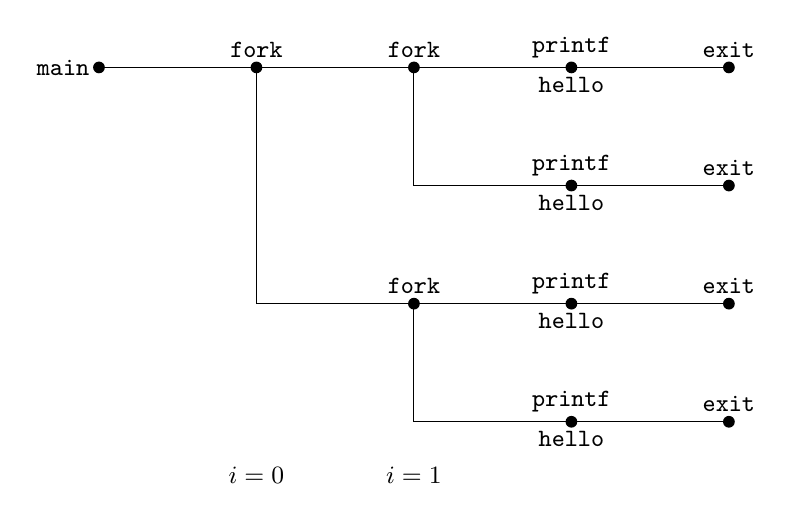
\begin{tikzpicture}[
  y=1.5cm,
  dot/.style={circle, fill, inner sep=1.5pt},
  lbl/.style={above, font=\small\ttfamily},
  output/.style={below, font=\small\ttfamily}
]
  % parent
  \draw (0,0) -- (8,0);
  \node[dot] at (0,0) {};
  \node[dot] at (2,0) {}; \node[lbl] at (2,0) {fork};
  \node[dot] at (4,0) {}; \node[lbl] at (4,0) {fork};
  \node[dot] at (6,0) {}; \node[lbl] at (6,0) {printf}; \node[output] at (6,0) {hello};
  \node[dot] at (8,0) {}; \node[lbl] at (8,0) {exit};

  % child of parent's second fork
  \draw (4,0) -- (4,-1);
  \draw (4,-1) -- (8,-1);
  \node[dot] at (6,-1) {}; \node[lbl] at (6,-1) {printf}; \node[output] at (6,-1) {hello};
  \node[dot] at (8,-1) {}; \node[lbl] at (8,-1) {exit};

  % child of parent's first fork
  \draw (2,0) -- (2,-2);
  \draw (2,-2) -- (8,-2);
  \node[dot] at (4,-2) {}; \node[lbl] at (4,-2) {fork};
  \node[dot] at (6,-2) {}; \node[lbl] at (6,-2) {printf}; \node[output] at (6,-2) {hello};
  \node[dot] at (8,-2) {}; \node[lbl] at (8,-2) {exit};

  % grandchild
  \draw (4,-2) -- (4,-3);
  \draw (4,-3) -- (8,-3);
  \node[dot] at (6,-3) {}; \node[lbl] at (6,-3) {printf}; \node[output] at (6,-3) {hello};
  \node[dot] at (8,-3) {}; \node[lbl] at (8,-3) {exit};

  \node[left, font=\small\ttfamily] at (0,0) {main};
  \node[below, font=\small] at (2,-3.3) {$i=0$};
  \node[below, font=\small] at (4,-3.3) {$i=1$};
\end{tikzpicture}
\end{center}

%===================== Problem 3 =====================
\item 8

\begin{center}
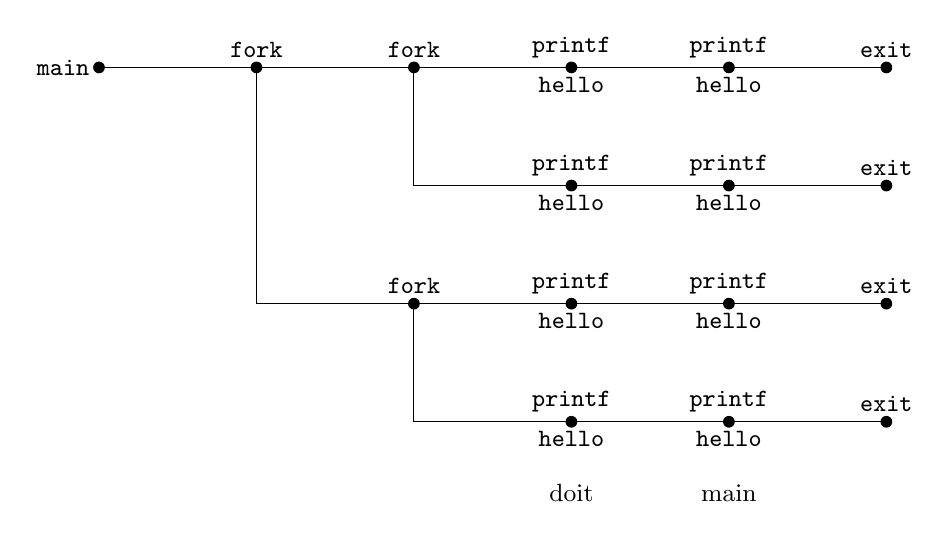
\begin{tikzpicture}[
  y=1.5cm,
  dot/.style={circle, fill, inner sep=1.5pt},
  lbl/.style={above, font=\small\ttfamily},
  output/.style={below, font=\small\ttfamily}
]
  % P
  \draw (0,0) -- (10,0);
  \node[dot] at (0,0) {};
  \node[dot] at (2,0) {}; \node[lbl] at (2,0) {fork};
  \node[dot] at (4,0) {}; \node[lbl] at (4,0) {fork};
  \node[dot] at (6,0) {}; \node[lbl] at (6,0) {printf}; \node[output] at (6,0) {hello};
  \node[dot] at (8,0) {}; \node[lbl] at (8,0) {printf}; \node[output] at (8,0) {hello};
  \node[dot] at (10,0) {}; \node[lbl] at (10,0) {exit};

  % C2 (P's second fork)
  \draw (4,0) -- (4,-1);
  \draw (4,-1) -- (10,-1);
  \node[dot] at (6,-1) {}; \node[lbl] at (6,-1) {printf}; \node[output] at (6,-1) {hello};
  \node[dot] at (8,-1) {}; \node[lbl] at (8,-1) {printf}; \node[output] at (8,-1) {hello};
  \node[dot] at (10,-1) {}; \node[lbl] at (10,-1) {exit};

  % C1 (P's first fork)
  \draw (2,0) -- (2,-2);
  \draw (2,-2) -- (10,-2);
  \node[dot] at (4,-2) {}; \node[lbl] at (4,-2) {fork};
  \node[dot] at (6,-2) {}; \node[lbl] at (6,-2) {printf}; \node[output] at (6,-2) {hello};
  \node[dot] at (8,-2) {}; \node[lbl] at (8,-2) {printf}; \node[output] at (8,-2) {hello};
  \node[dot] at (10,-2) {}; \node[lbl] at (10,-2) {exit};

  % C3 (C1's fork)
  \draw (4,-2) -- (4,-3);
  \draw (4,-3) -- (10,-3);
  \node[dot] at (6,-3) {}; \node[lbl] at (6,-3) {printf}; \node[output] at (6,-3) {hello};
  \node[dot] at (8,-3) {}; \node[lbl] at (8,-3) {printf}; \node[output] at (8,-3) {hello};
  \node[dot] at (10,-3) {}; \node[lbl] at (10,-3) {exit};

  \node[left, font=\small\ttfamily] at (0,0) {main};
  \node[below, font=\small] at (6,-3.45) {doit};
  \node[below, font=\small] at (8,-3.45) {main};
\end{tikzpicture}
\end{center}

%===================== Problem 4 =====================
\item
\begin{Verbatim}
Parent (Fork() != 0):  x = 3  ->  ++x = 4 (print)  ->  --x = 3 (print)
Child  (Fork() == 0):  x = 3  ->  --x = 2 (print)
\end{Verbatim}

Output:
\begin{Verbatim}
x=4
x=3
x=2
\end{Verbatim}

%===================== Problem 5 =====================
\item
\begin{Verbatim}
Child  (fork() == 0):  counter = 1  ->  counter-- = 0  ->  exit (no print)
Parent (fork() != 0):  counter = 1  ->  Wait  ->  ++counter = 2 (print)
\end{Verbatim}

Output:
\begin{Verbatim}
counter = 2
\end{Verbatim}

\end{enumerate}

\end{document}
